\chapter{Connector Pinouts}
\section{RS-485 Connection (terminal block J1)}
\begin{center}
	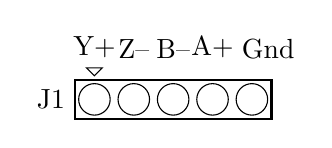
\begin{tikzpicture}[scale=.5]
		\draw [thick] (.5,.5) -- (5.5,.5) -- (5.5,1.5) -- (.5,1.5) -- cycle;
		\foreach \x in {1, 2, 3, 4, 5} {
			\draw (\x,1) circle (.4);
		}
		\node [above] at (1,1.8) {Y+};
		\node [above] at (2,1.8) {Z--};
		\node [above] at (3,1.8) {B--};
		\node [above] at (4,1.8) {A+};
		\node [above right] at (4.5,1.8) {Gnd};
		\node [left] at (.5,1) {J1};
		%\node [right] at (5.5,1) {J9};
		\draw (1,1.6) -- (0.8,1.8) -- (1.2,1.8) -- cycle;
	\end{tikzpicture}
\end{center}
Note that \acronym{RS-485} works best if the signal bus is a single line from one end to the other, with
very short ``taps'' in the line for each Lumos board.  In other words, if this is one unit in a chain, both
the input and output lines should be tied to the terminal block.  Do not ``tap in'' to the communication line and run
a single jumper out to the Lumos board.

If this is the last device in the chain, install a terminator at R14.

The main data line carrying \acronym{PC} commands to the Lumos boards connects at ``A+'' and ``B--'' (the positive
and negative signals respectively).  The return channel (for full-duplex networks) is on ``Y+'' and ``Z--''.

\section{Sensor Input Terminals (J0)}
\begin{center}
	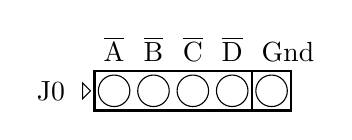
\begin{tikzpicture}[scale=.5]
		\draw [thick] (.5,.5) -- (5.5,.5) -- (5.5,1.5) -- (.5,1.5) -- cycle;
		\foreach \x in {1, 2, 3, 4, 5} {
			\draw (\x,1) circle (.4);
		}
		\draw [thick] (4.5, .5) -- (4.5, 1.5);
		\node [above] at (1,1.5) {$\overline{\hbox{A}}$};
		\node [above] at (2,1.5) {$\overline{\hbox{B}}$};
		\node [above] at (3,1.5) {$\overline{\hbox{C}}$};
		\node [above] at (4,1.5) {$\overline{\hbox{D}}$};
		\node [above right] at (4.5,1.5) {Gnd};
		\node [left] at (0,1) {J0};
		%\node [right] at (5.5,1) {J9};
		\draw (0.4,1) -- (0.2,1.2) -- (0.2,0.8) -- cycle;
	\end{tikzpicture}
\end{center}
If the Lumos controller is built to accommodate one or more sensor inputs, a set of terminals will be installed
at J0.  

It is important to note that the board's circuitry must be configured for certain inputs to be enabled
at the time the board is built, and that the board must be configured (using software) to recognize those
inputs, before they will be usable.

Each input accepts a \acronym{TTL}-level signal.  The lines are pulled up to +5\,V internally.  The board
can be configured in software to react to the inputs as active-high or active-low.

%\input dutycycle

\section{Control/ICSP Header (J2)}
\begin{center}
	
\begin{tikzpicture}[scale=.5]
		\draw [line width=10] (-.6,1)--(5.4,1);
		\foreach \x in {0, 1, 2, 3, 4, 5} {
			\foreach \y in {1} {
				\draw [fill=white] (\x-.2,\y-.2) -- (\x-.2,\y+.2) -- (\x+.2,\y+.2) -- (\x+.2,\y-.2) -- cycle;
			}
		}
		\draw (5.5,1) -- (6,1.25) -- (6,0.75) -- cycle;
		\node [above] at (0,1.5) {6};
		\node [above] at (1,1.5) {5};
		\node [above] at (2,1.5) {4};
		\node [above] at (3,1.5) {3};
		\node [above] at (4,1.5) {2};
		\node [above] at (5,1.5) {1};
		\node [right] at (7, 3.0) {1 $\hbox{V}_{\hbox{\footnotesize DD}}$ (+5\,V)};
		\node [right] at (7, 2.0) {2 $\hbox{V}_{\hbox{\footnotesize SS}}$ (Ground)};
		\node [right] at (7, 1.0) {3 $\hbox{V}_{\hbox{\footnotesize PP}}/\overline{\hbox{\mc{MCLR}}}/\overline{\hbox{\mc{RESET}}}$};
		\node [right] at (15, 3.0) {4 PGD$/\overline{\hbox{\mc{PWR CTL}}}$};
		\node [right] at (15, 2.0) {5 PGC$/\overline{\hbox{\mc{OPTION}}}$};
		\node [right] at (15, 1.0) {6 Ground};
	\end{tikzpicture}
\end{center}

This header is used for reprogramming a new firmware image onto the microcontroller chip.  Be sure to check the pinout
used by your programmer before connecting it to this port.  It may be different!

During normal operations, this header may also be used to connect off-board buttons for the reset and option functions.  
These buttons should be normally open, but connect their respective pins to ground when pushed. 
Note that the $\overline{\hbox{\mc{PWR CTL}}}$ output is only available on this header.  If the board is to be used
with a controlled power supply, a connector will need to be used to obtain this signal from J2.

\section{Voltage Select Headers (J3, J4)}\label{sec:voltagesw}
\begin{center}
	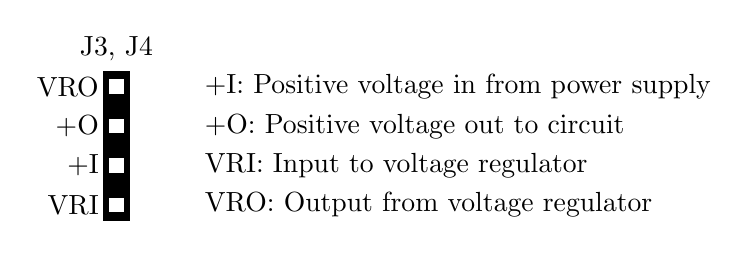
\begin{tikzpicture}[scale=.5]
		%\draw [line width=10] (.6,1)--(4.4,1);
		%\draw [line width=10] (1,.6)--(1,4.4);
		\draw [line width=10] (5,.6)--(5,4.4);
		\foreach \y in {1, 2, 3, 4} {
			\foreach \x in {5} {
				\draw [fill=white] (\x-.2,\y-.2) -- (\x-.2,\y+.2) -- (\x+.2,\y+.2) -- (\x+.2,\y-.2) -- cycle;
			}
		}
		%\node [above] at (1,4.4) {J17};
		\node [above] at (5,4.4) {J3, J4};
		%\node [left] at (.8,1) {VRO};
		%\node [left] at (.8,2) {+O};
		%\node [left] at (.8,3) {+I};
		%\node [left] at (.8,4) {VRI};
		\node [left] at (4.8,1) {VRI};
		\node [left] at (4.8,2) {+I};
		\node [left] at (4.8,3) {+O};
		\node [left] at (4.8,4) {VRO};

		\node [right] at (7, 4) {+I: Positive voltage in from power supply};
		\node [right] at (7, 3) {+O: Positive voltage out to circuit};
		\node [right] at (7, 2) {VRI: Input to voltage regulator};
		\node [right] at (7, 1) {VRO: Output from voltage regulator};
	\end{tikzpicture}
\end{center}
J3 and J4 
are used to select the input voltage supplied to the load power control and the logic portion of the board.
The square pin on the board corresponds to the VCO pin in the diagram above.
If a regulated +5\,V supply is employed, there is no
need for the on-board regulator (and in fact it can't function properly unless its input is at least +8\,V), so a jumper
is placed across the middle two pins (connecting +I and +O), bypassing the voltage regulator entirely.  \emph{In this 
case, it is critically important that the input voltage be a clean, regulated +5\,V supply.  If this voltage is exceeded,
permanent damage to the Lumos board will result!}

If +8\,V to +24\,V is attached to an input, the corresponding jumper block needs jumpers installed into the outer two pins,
connecting +I to VRI and +O to VRO.  This routes the incoming power through the voltage regulator.
